\chapter{Экспериментальная часть}

В данном разделе будет произведено сравнение двух алгоритмов:

\begin{enumerate}
	\item полный перебор;
	\item муравьиный алгоритм.
\end{enumerate}

\section{Сравнение времени работы муравьиного алгоритма и полного перебора}

Для сравнения возьмем 8 массивов городов размерностью
$[$3, 4, 5, 6, 7, 8, 9, 10$]$.
Воспользуемся усреднением массового эксперимента.

Результат сравнения муравьиного алгоритма и полного перебора представлен на рис. \ref{ref:time}.

\begin{figure}[ht!]
	\centering{
		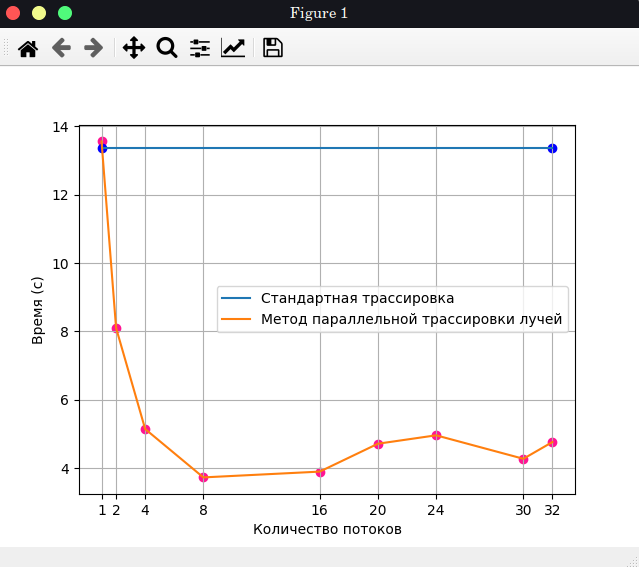
\includegraphics[width=0.8\textwidth]{time.png}
		\caption{Время работы муравьиного алгоритма и полного перебора}
		\label{ref:time}}
\end{figure}

По результатам эксперимента видно, что время испольнения муравьиного алгоритма
значительно меньше, чем исполнение алгоритма полного перебора.

\newpage

\section{Результат работы программы}

На рисунках \ref{ref:res1} -- \ref{ref:res3} приведены результаты работы программы.
Синим цветом показан путь, который нашел муравьиный алгоритм.
Красным цветом показан путь, найденный полным перебором.
На рисунке \ref{ref:res2} показана ситуация, когда муравьиный алгоритм ошибся.
Также на рисунке \ref{ref:res3} показан вывод в консоль.

\begin{figure}[ht!]
	\centering{
		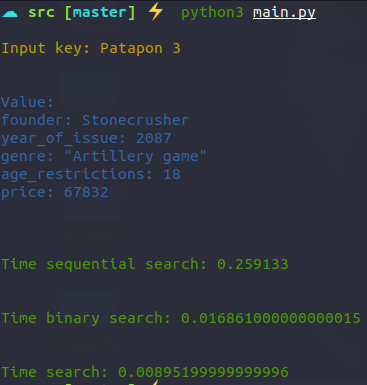
\includegraphics[width=1\textwidth]{res1.png}
		\caption{Результат работы программы}
		\label{ref:res1}}
\end{figure}

\begin{figure}[ht!]
	\centering{
		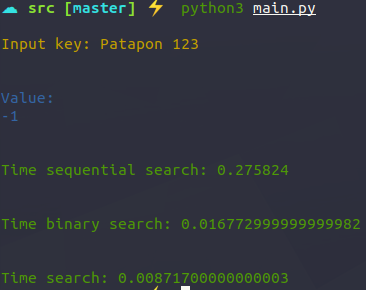
\includegraphics[width=1\textwidth]{res2.png}
		\caption{Результат работы программы}
		\label{ref:res2}}
\end{figure}


\begin{figure}[ht!]
	\centering{
		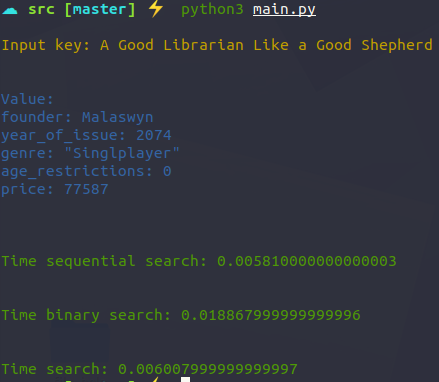
\includegraphics[width=0.7\textwidth]{res3.png}
		\caption{Результат работы программы}
		\label{ref:res3}}
\end{figure}


\newpage

\section{Параметризация муравьиного алгоритма}

В муравьином алгоритме вычисления производятся на основе настраиваемых параметров.

Рассмотрим матрицу смежностей размерностью $10\times10$ (\ref{table:matrix})

\begin{table}[ht]
	\centering
	\caption{Матрица смежностей}
	\label{table:matrix}
	\begin{tabular}{ | l | l | l | l | l | l | l | l | l | l | l |}
		\hline
		0 & 0    & 1    & 2    & 3    & 4    & 5    & 6    & 7    & 8    & 9    \\ \hline
		0 & 0    & 1790 & 200  & 1900 & 63   & 1659 & 1820 & 1395 & 2382 & 649  \\ \hline
		1 & 1790 & 0    & 1573 & 2435 & 1515 & 714  & 892  & 2193 & 1590 & 1003 \\ \hline
		2 & 200  & 1573 & 0    & 833  & 392  & 2404 & 962  & 902  & 141  & 1123 \\ \hline
		3 & 1900 & 2435 & 833  & 0    & 2283 & 1652 & 2362 & 2262 & 1512 & 2166 \\ \hline
		4 & 63   & 1515 & 392  & 2283 & 0    & 1322 & 290  & 1305 & 2100 & 969  \\ \hline
		5 & 1659 & 714  & 2404 & 1652 & 1322 & 0    & 256  & 78   & 2236 & 2041 \\ \hline
		6 & 1820 & 892  & 962  & 2362 & 290  & 256  & 0    & 1180 & 1547 & 1279 \\ \hline
		7 & 1395 & 2193 & 902  & 2262 & 1305 & 78   & 1180 & 0    & 1640 & 1161 \\ \hline
		8 & 2382 & 1590 & 141  & 1512 & 2100 & 2236 & 1547 & 1640 & 0    & 2212 \\ \hline
		9 & 649  & 1003 & 1123 & 2166 & 969  & 2041 & 1279 & 1161 & 2212 & 0    \\ \hline
	\end{tabular}
\end{table}

\newpage


\begin{table}[ht]
	\centering
	\caption{Таблица коэффициентов.Часть 1}
	\label{table:ref1}
	\begin{tabular}{ | l | l | l | l | l |}
		\hline
		$\alpha$ & $\beta$ & p   & Результат & Разница \\
		\hline
		0        & 1       & 0   & 6986      & 0       \\
		0        & 1       & 0.1 & 6986      & 0       \\
		0        & 1       & 0.2 & 6986      & 0       \\
		0        & 1       & 0.3 & 6986      & 0       \\
		0        & 1       & 0.4 & 6986      & 0       \\
		0        & 1       & 0.5 & 6986      & 0       \\
		0        & 1       & 0.6 & 6986      & 0       \\
		0        & 1       & 0.7 & 6986      & 0       \\
		0        & 1       & 0.8 & 6986      & 0       \\
		0        & 1       & 0.9 & 6992      & 6       \\
		0        & 1       & 1   & 6986      & 0       \\
		0.1      & 0.9     & 0   & 6986      & 0       \\
		0.1      & 0.9     & 0.1 & 6992      & 6       \\
		0.1      & 0.9     & 0.2 & 6986      & 0       \\
		0.1      & 0.9     & 0.3 & 6986      & 0       \\
		0.1      & 0.9     & 0.4 & 6986      & 0       \\
		0.1      & 0.9     & 0.5 & 6986      & 0       \\
		0.1      & 0.9     & 0.6 & 6986      & 0       \\
		0.1      & 0.9     & 0.7 & 6986      & 0       \\
		0.1      & 0.9     & 0.8 & 6986      & 0       \\
		0.1      & 0.9     & 0.9 & 7165      & 179     \\
		0.1      & 0.9     & 1   & 6986      & 0       \\
		0.2      & 0.8     & 0   & 6986      & 0       \\
		0.2      & 0.8     & 0.1 & 6986      & 0       \\
		0.2      & 0.8     & 0.2 & 6986      & 0       \\
		0.2      & 0.8     & 0.3 & 6992      & 6       \\
		0.2      & 0.8     & 0.4 & 6992      & 6       \\
		0.2      & 0.8     & 0.5 & 6992      & 6       \\
		0.2      & 0.8     & 0.6 & 6986      & 0       \\
		0.2      & 0.8     & 0.7 & 6992      & 6       \\
		0.2      & 0.8     & 0.8 & 6986      & 0       \\
		0.2      & 0.8     & 0.9 & 6986      & 0       \\
		0.2      & 0.8     & 1   & 6986      & 0       \\
		\hline
	\end{tabular}
\end{table}

\begin{table}[ht]
	\centering
	\caption{Таблица коэффициентов.Часть 2}
	\label{table:ref2}
	\begin{tabular}{ | l | l | l | l | l |}
		\hline
		$\alpha$ & $\beta$ & p   & Результат & Разница \\
		\hline
		0.3      & 0.7     & 0   & 6986      & 0       \\
		0.3      & 0.7     & 0.1 & 6986      & 0       \\
		0.3      & 0.7     & 0.2 & 7139      & 153     \\
		0.3      & 0.7     & 0.3 & 7139      & 153     \\
		0.3      & 0.7     & 0.4 & 6986      & 0       \\
		0.3      & 0.7     & 0.5 & 6986      & 0       \\
		0.3      & 0.7     & 0.6 & 6986      & 0       \\
		0.3      & 0.7     & 0.7 & 6986      & 0       \\
		0.3      & 0.7     & 0.8 & 6992      & 6       \\
		0.3      & 0.7     & 0.9 & 6992      & 6       \\
		0.3      & 0.7     & 1   & 6986      & 0       \\
		0.4      & 0.6     & 0   & 6986      & 0       \\
		0.4      & 0.6     & 0.1 & 6992      & 6       \\
		0.4      & 0.6     & 0.2 & 6986      & 0       \\
		0.4      & 0.6     & 0.3 & 6986      & 0       \\
		0.4      & 0.6     & 0.4 & 6986      & 0       \\
		0.4      & 0.6     & 0.5 & 6992      & 6       \\
		0.4      & 0.6     & 0.6 & 6992      & 6       \\
		0.4      & 0.6     & 0.7 & 6986      & 0       \\
		0.4      & 0.6     & 0.8 & 7139      & 153     \\
		0.4      & 0.6     & 0.9 & 6986      & 0       \\
		0.4      & 0.6     & 1   & 6992      & 6       \\
		0.5      & 0.5     & 0   & 7139      & 153     \\
		0.5      & 0.5     & 0.1 & 6986      & 0       \\
		0.5      & 0.5     & 0.2 & 6986      & 0       \\
		0.5      & 0.5     & 0.3 & 7139      & 153     \\
		0.5      & 0.5     & 0.4 & 6986      & 0       \\
		0.5      & 0.5     & 0.5 & 6986      & 0       \\
		0.5      & 0.5     & 0.6 & 6986      & 0       \\
		0.5      & 0.5     & 0.7 & 6986      & 0       \\
		0.5      & 0.5     & 0.8 & 6986      & 0       \\
		0.5      & 0.5     & 0.9 & 6986      & 0       \\
		0.5      & 0.5     & 1   & 6986      & 0       \\

		\hline
	\end{tabular}
\end{table}


\begin{table}[ht]
	\centering
	\caption{Таблица коэффициентов.Часть 3}
	\label{table:ref3}
	\begin{tabular}{ | l | l | l | l | l |}
		\hline
		$\alpha$ & $\beta$ & p   & Результат & Разница \\
		\hline
		0.6      & 0.4     & 0   & 7139      & 153     \\
		0.6      & 0.4     & 0.1 & 6992      & 6       \\
		0.6      & 0.4     & 0.2 & 6986      & 0       \\
		0.6      & 0.4     & 0.3 & 6986      & 0       \\
		0.6      & 0.4     & 0.4 & 7139      & 153     \\
		0.6      & 0.4     & 0.5 & 6992      & 6       \\
		0.6      & 0.4     & 0.6 & 6986      & 0       \\
		0.6      & 0.4     & 0.7 & 6986      & 0       \\
		0.6      & 0.4     & 0.8 & 6986      & 0       \\
		0.6      & 0.4     & 0.9 & 6992      & 6       \\
		0.6      & 0.4     & 1   & 6986      & 0       \\
		0.7      & 0.3     & 0   & 6986      & 0       \\
		0.7      & 0.3     & 0.1 & 6986      & 0       \\
		0.7      & 0.3     & 0.2 & 6986      & 0       \\
		0.7      & 0.3     & 0.3 & 7139      & 153     \\
		0.7      & 0.3     & 0.4 & 7165      & 179     \\
		0.7      & 0.3     & 0.5 & 7139      & 153     \\
		0.7      & 0.3     & 0.6 & 6992      & 6       \\
		0.7      & 0.3     & 0.7 & 6992      & 6       \\
		0.7      & 0.3     & 0.8 & 6986      & 0       \\
		0.7      & 0.3     & 0.9 & 6992      & 6       \\
		0.7      & 0.3     & 1   & 6986      & 0       \\
		0.8      & 0.2     & 0   & 7139      & 153     \\
		0.8      & 0.2     & 0.1 & 7562      & 576     \\
		0.8      & 0.2     & 0.2 & 6992      & 6       \\
		0.9      & 0.1     & 0.2 & 6992      & 6       \\
		0.9      & 0.1     & 0.3 & 6986      & 0       \\
		0.9      & 0.1     & 0.4 & 7139      & 153     \\
		0.9      & 0.1     & 0.5 & 7329      & 343     \\
		0.9      & 0.1     & 0.6 & 7217      & 231     \\
		0.9      & 0.1     & 0.7 & 7139      & 153     \\
		0.9      & 0.1     & 0.8 & 7217      & 231     \\
		0.9      & 0.1     & 0.9 & 7376      & 390     \\
		0.9      & 0.1     & 1   & 6986      & 0       \\
		\hline
	\end{tabular}
\end{table}


\begin{table}[ht]
	\centering
	\caption{Таблица коэффициентов.Часть 4}
	\label{table:ref4}
	\begin{tabular}{ | l | l | l | l | l |}
		\hline
		$\alpha$ & $\beta$ & p   & Результат & Разница \\
		\hline
		1        & 0       & 0   & 8531      & 1545    \\
		1        & 0       & 0.1 & 8588      & 1602    \\
		1        & 0       & 0.2 & 6986      & 0       \\
		1        & 0       & 0.3 & 7720      & 734     \\
		1        & 0       & 0.4 & 7554      & 568     \\
		1        & 0       & 0.5 & 6992      & 6       \\
		1        & 0       & 0.6 & 7920      & 934     \\
		1        & 0       & 0.7 & 7217      & 231     \\
		1        & 0       & 0.8 & 7874      & 888     \\
		1        & 0       & 0.9 & 7446      & 460     \\
		1        & 0       & 1   & 8119      & 1133    \\
		\hline
	\end{tabular}
\end{table}

\newpage

Параметризация метода решения задачи коммивояжера
на основании муравьиного алгоритма проводилась для матрицы с
элементами в диапозоне [0, 2500].
Количество дней было равно 50.
Полный перебор определил оптимальную длину пути 6986.
Столбец ''результат'' отвечает за результат работы муравьиного алгоритма.
Столбец ''разница'' отвечает за разницу с оптимальной длиной.




\section{Вывод}

На основе проведенной параметризации (таблицы \ref{table:ref1}--\ref{table:ref4}) для матрицы смежности
приведенной в таблице (\ref{table:matrix}) рекомендуется использовать
$(\alpha = 0.5, \beta = 0.5, \rho = \text{любое})$.
При этих параметрах, количество правильно найденных оптимальных путей составило 8 единиц.

% В данном разделе было произведено сравнение
% последовательной реализации трех алгоритмов
% и конвейера с использованием многопоточности.
% По результатам исследования конвейерную обработку
% нет смысла применять на задачах, занимающих мало времени.
% Статистика показала, что конвейерная обработка работает правильно.